\section{Query answering with optimal snapshots}

In this section we will discuss the evaluation of query workloads with the
database given in Section~\ref{sec:trusted-db}.  Each table $\Hat T$ is a timeline of
transactions, digitally signed and verifiable.  Recall in
Section~\ref{sec:problem-def}, we need to process a large number of queries at
different query timestamps.

To support arbitrary query $q$, we need to compute the snapshots of all the tables
$\Hat{T}$ that are needed by $q$ at $t_q$. This means we need to perform
a group-by operation using the row id (from the original table $T$), with each
group aggregated to the
row with the latest transaction timestamp.  Then we remove all the rows with
their deletion boolean flags set to true.
This can be expressed in SQL using windowing functions as shown in
Figure~\ref{fig:sql}.

Finally, the query $q$ is evaluated as:
$q(\mathrm{snapshot}(\Hat T_1, t_q), \mathrm{snapshot}(\Hat T_2, t_q), \dots)$.

\begin{figure}[h]
\centering
\begin{tabular}{l} \hline \hline
$\mathrm{snapshot}(\Hat T, t_q)$: \\ \hline
\verb|  |WITH $V$ AS ( \\
\verb|    |SELECT id, \{last\_value($x$) : $x\in\attr(T)$\} OVER $W$ \\
\verb|    |FROM $\Hat T$ \\
\verb|    |WHERE $\Hat T.t \leq t_q$ \\
\verb|    |WINDOW $W$ AS PARTITION BY id ORDER BY $\Hat T.t$ \\
\verb|  |)
\verb|  |SELECT id, $\{x: x\in\attr(T)\}$ \\
\verb|  |FROM $V$ \\
\verb|  |WHERE NOT $V.\mathrm{del?}$ \\ \hline \hline
\end{tabular}
\caption{Aggregation query to generate the snapshot of a time at a given
timestamp.}
\label{fig:sql}
\end{figure}

For the remainder of this section, we present a family of optimization
techniques to efficiently process query workload $Q = \{q_1, q_2, \dots, q_N\}$
by optimally materialize a fixed number of snapshots.

\subsection{Materialized single snapshot}

\newcommand{\snapshot}{\mathrm{snapshot}}
\newcommand{\cost}{\mathrm{cost}}
\newcommand{\opt}{\mathrm{opt}}

If we have a snapshot $S = \mathrm{snapshot}(T, t_s)$, and a query $q$ with
query timestamp $t_q\not t_s$, we can evaluate $q$ by
constructing $\snapshot(T, t_q)$ based on $S$.  This involves applying all the
transactions in the interval of $[t_s, t_q]$ (commit transactions) or $[t_q,
t_s]$ (rollback transactions). Since each transaction has its unique timestamp,
the number of transactions in the interval is given by $|t_q - t_s|$.

Suppose we only have a single materialized snapshot $s$, and a query workload
$Q$.  When every query $q\in Q$ utilizes $s$ to compute $\snapshot(S, t_q)$,
we have the following cost model:
$$\cost(Q|s) = \sum_{q\in Q} |t_q - t_s|$$

This leads to the first optimization problem.

\newcommand{\argmin}[1]{\underset{#1}{\mathrm{argmin}\ }}

\begin{definition}[Optimal single snapshot placement problem]
    Given a query workload, What is is an optimal snapshot placement $s^*$ where
    $s^* = \argmin{s}\cost(Q|s)$?
\end{definition}

One can show that the single snapshot placement can be solved by placing the
snapshot at the median of the query timestamps.

\begin{theorem}[Optimal single snapshot placement]
    $$ t_s^* = \mathrm{median}(t_q : q\in Q) $$
    \label{thm:single}
\end{theorem}

\subsection{Materializing multiple snapshots}

Naturally, we expect to improve the performance with multiple snapshots.  This
takes us to the multiple snapshot problem. Let $S = \{s_1, s_2, \dots, s_m\}$,
and $Q$ the query workload.  Each query will be evaluated using the {\em nearest} snapshot.
So, the cost becomes:

$$ \cost(Q|S) = \sum_{q\in Q} \min\{|t_q - t_s| : s\in S\} $$

\begin{definition}[Optimial m-snapshots placement problem]
    Let $S^* = \{s_1, s_2, \dots, s_m\}$ be $m$ snapshots.  What
    are the placements so that $\cost(Q|S)$ is minimized?
    We will denote $S^*$ as $\mathrm{opt}(Q, m)$.
\end{definition}

We first observe that the m-snapshot problem enjoys a property that we call the
{\em optimality of subproblems}.

\begin{theorem}[Optimality of subproblems]
    Let $S^* = \mathrm{opt}(Q, m)$.  Then $S^*$ partitions $Q$ by the nearest
    snapshot relation.  The prefix of $S^*$ is also an optimal snapshot
    placement of the prefix of the partition of $Q$.
    \label{thm:subproblem}
\end{theorem}

This leads to a recursive solution to the $m$-snapshot
placement problem shown in Figure~\ref{fig:recursion}.

\begin{figure}[htbp]
    \centering
    \begin{tabular}{l} \hline \hline
        Base case: \\
        \verb|  | $\opt(Q, 1) = \{\mathrm{median}(Q)\}$ \\ \hline
        Induction: \\
        \verb|  | let $i^* = \argmin{i\in[1,n]} \cost(\opt(Q[1:i], m-1))$ \\
        \verb|  | let $n = |Q|$ \\
        \verb|  | $\opt(Q, m) = \opt(Q[1:i^*]) \cup \{\mathrm{median}(Q[i^*+1:n])$ \\
        \hline \hline
    \end{tabular}
    \caption{Recursive solution to the $m$-snapshot placement problem.}
    \label{fig:recursion}
\end{figure}

It can be shown that the recursion in Figure~\ref{fig:recursion} can be
implemented as dynamic programming with complexity $\mathcal{O}(mn^2)$
where $m$ is the number of snapshots, and $n$ the number of queries.

\subsection{Approximate snapshot placement using clustering}

While the algorithm in Figure~\ref{fig:recursion} computes the optimal snapshot
placement in polynomial time, its complexity is still too high if the query load is
large (thousands) with many materialized snapshots (hundreds).

We make the observation that the optimal $m$-snapshot placement is based on
the medians of subsets of queries.  This is also true
for the case of $m=1$ as given in Theorem~\ref{thm:single}.
This leads us to believe that the cluster structure in the timestamps of the
query workload is a strong determining factor in snapshot placement.  Thus, we
propose to {\em approximate} the optimal snapshot locations by the {\em mean}
centroids of $m$-clustering of $\{t_q : q\in Q\}$ as shown in
Figure~\ref{fig:approx}.

\begin{figure}[htbp]
    \centering
    \begin{tabular}{l}\hline\hline
        $\mathrm{approx}(Q, m)$: \\ \hline
        \verb|  | $\mathbf{C} = \textrm{k-mean-clustering}(\{t_q: q\in Q\}, m)$ \\
        \verb|  | return $\{\mathrm{mean}(C) : C\in\mathbf{C}\}$ \\ \hline\hline
    \end{tabular}
    \caption{Approximate snapshot placements using clustering}
    \label{fig:approx}
\end{figure}
\begin{figure}[b] 
    \centering 
    \subfloat[Answering a single query using the nearest snapshots] { 
    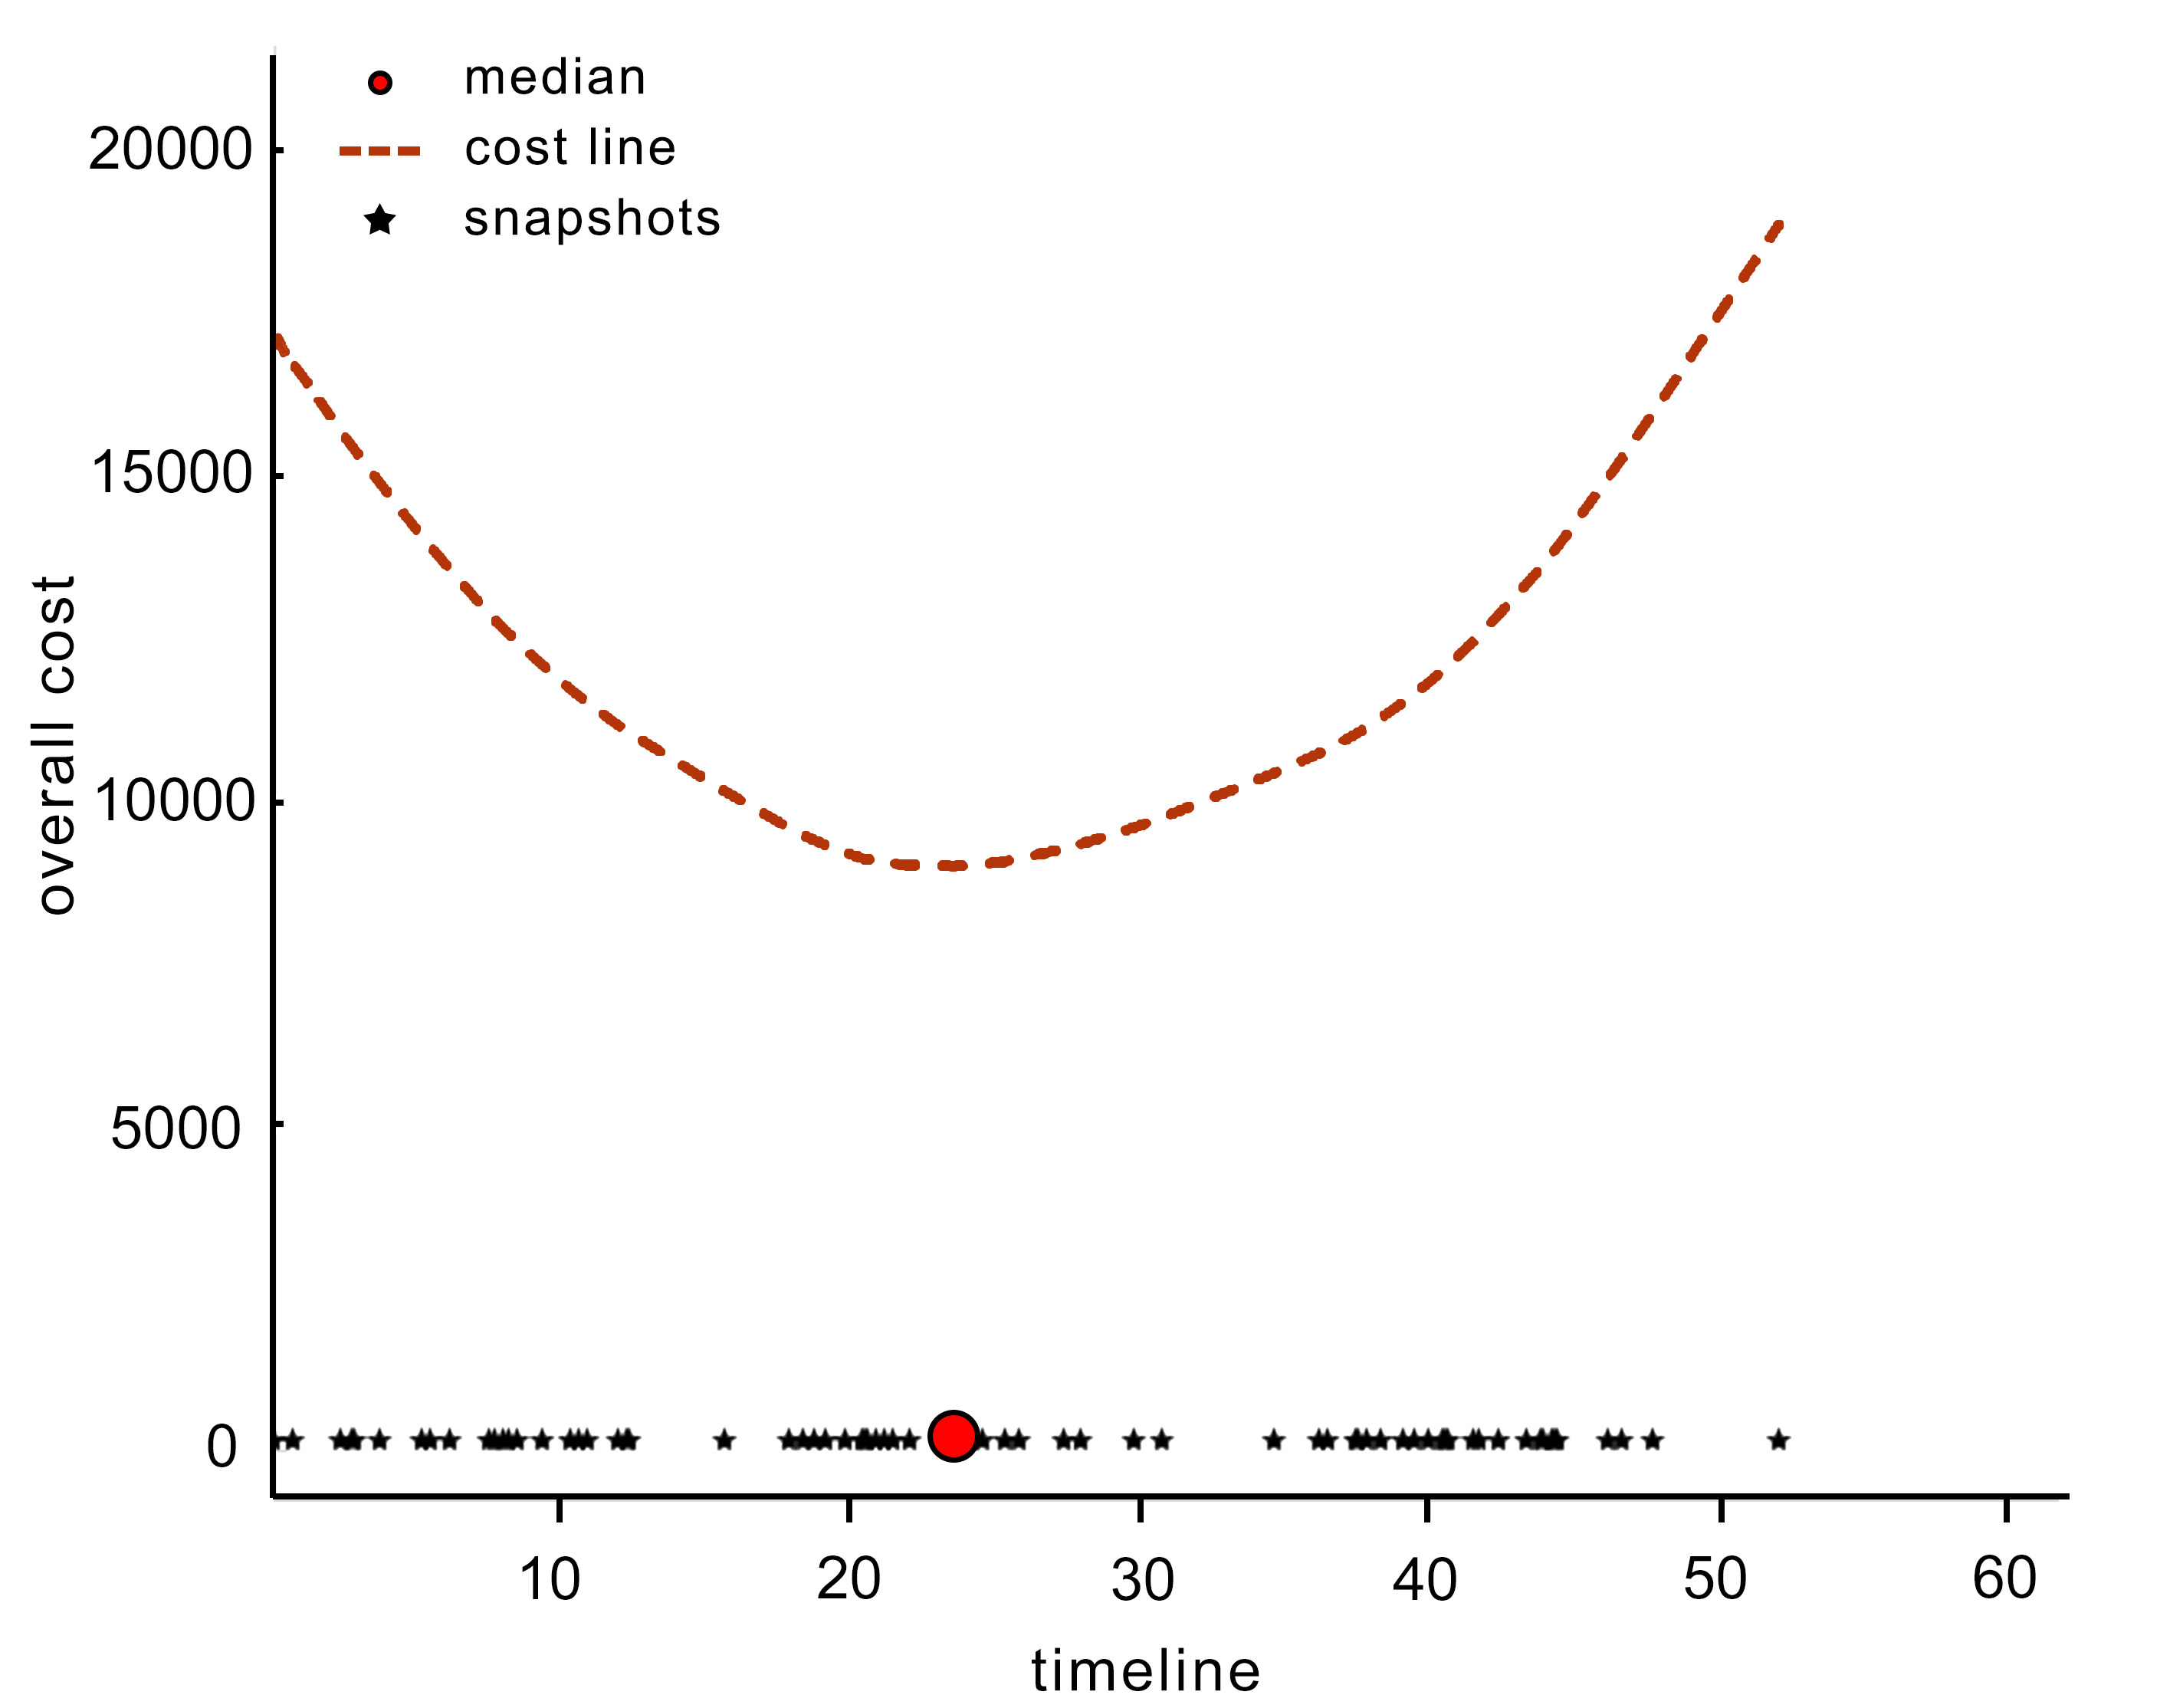
\includegraphics[width=0.3\linewidth]{figs/single_snapshot.jpg}
    \label{fig:query-answer-1}
    }
    \hfill 
    \subfloat[Reduction in cost with increasing number of snapshots]{
    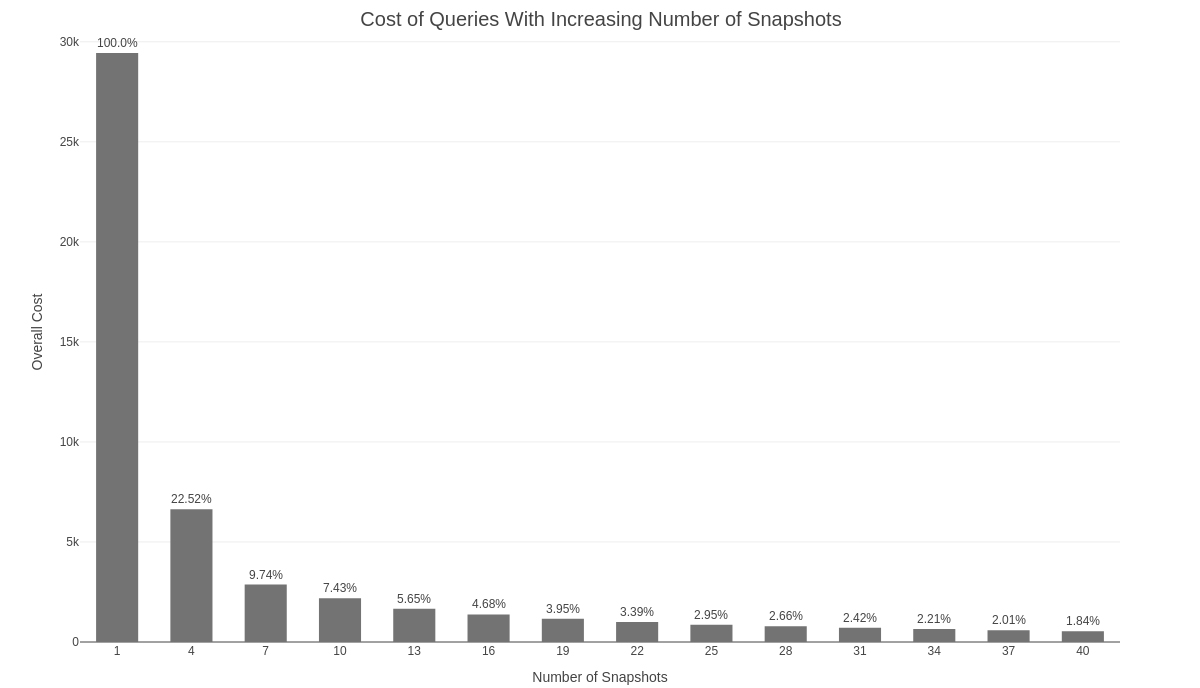
\includegraphics[width=0.3\linewidth]{figs/various_snapshot.jpg} 
    \label{fig:query-answer-3}
    }
    \hfill
    \subfloat[Different snapshot selection algorithms]{
    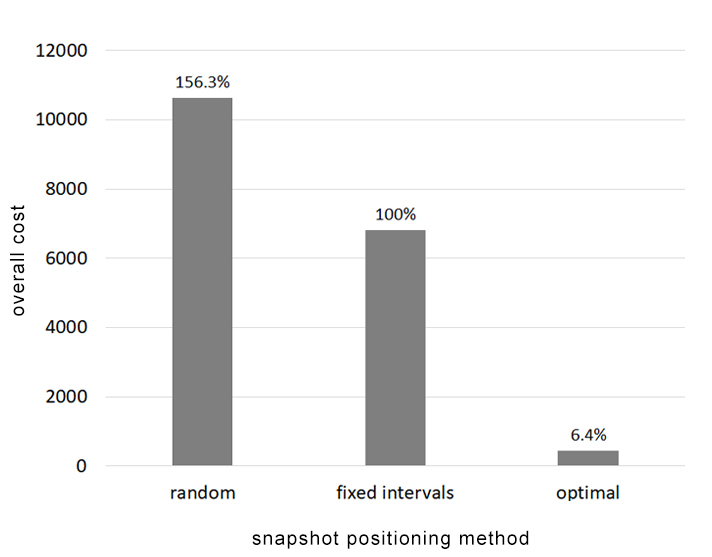
\includegraphics[width=0.3\linewidth]{figs/various_scenarios_cost.jpg} 
    \label{fig:query-answer-2}
    } 
    \caption{The effects of query workload answering using materialized snapshots}
    \label{fig:query-answer}
\end{figure}


\begin{figure}[t]
\centering
    \subfloat[Optimal vs heuristic runtime] {
    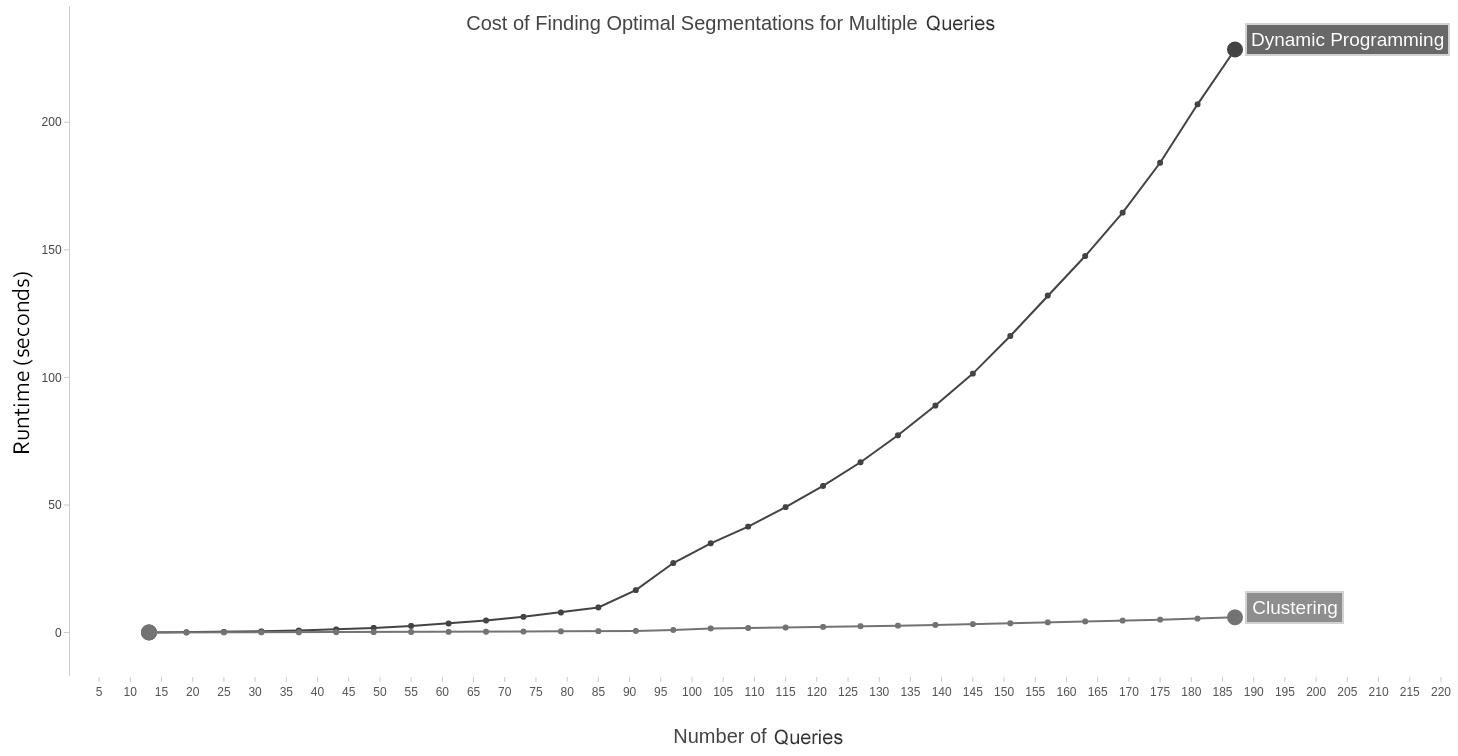
\includegraphics[width=0.45\linewidth]{figs/multi_query_2.jpg}
    \label{fig:runtime-1}
    }
    \hfill
    \subfloat[Heuristc with 300 iterations and 30 iterations] {
    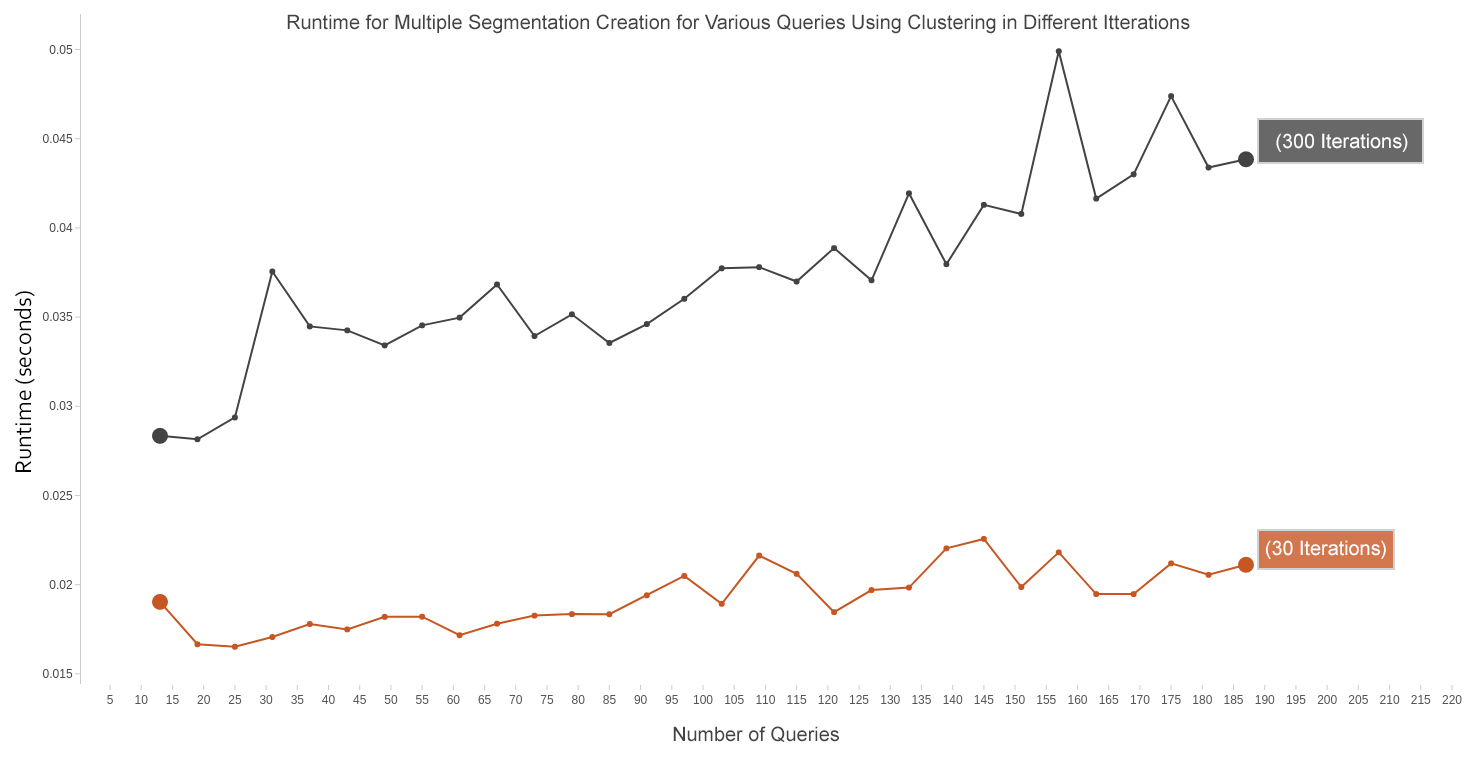
\includegraphics[width=0.45\linewidth]{figs/multiQuery_clustering.jpg}
    \label{fig:runtime-2}
    }
    \caption{Runtime comparision of different snapshot placements}
\end{figure}


This is encouraging since k-mean-clustering has a complexity of
$\mathcal{O}(mn)$.  In fact, we can also adjust the runtime by controlling the
number of iterations over the query timestamps.  By reducing the number of
iterations we can further speed up the snapshot placement computation.



